\documentclass[conference]{styles/acmsiggraph}

\usepackage{fullpage} % changes the margin
\usepackage{graphicx}
\usepackage[dvipsnames]{xcolor}
\usepackage{hyperref}
\usepackage{titlesec}
\usepackage{float}
\usepackage{booktabs}
\setlength{\parskip}{.8mm}

\pdfauthor{Vudavagandla Rohan, Verma Jatin}

\hypersetup{
	colorlinks=true,
}

\titlespacing*{\section}{0pt}{5.5ex plus 1ex minus .2ex}{2ex}
\titlespacing*{\subsection}{0pt}{3ex}{2ex}

\begin{document}

\begin{titlepage}
  \centering
  \vspace*{\fill}

  {\huge\bfseries Gossip and Push-Sum Simulator Report\par}
  \vspace{1em}
  {\LARGE COP5615 : Distributed Operating Systems Principles\par}
  \vspace{0.5em}
  {\large Professor Alin Dobra\par}
  \vspace{2em}
  {\Large Vudavagandla Rohan, Verma Jatin\par}
  \vspace{0.5em}
  {\normalsize vudavagandla.ro@ufl.edu, jverma@ufl.edu\par}

  \vspace*{\fill}
\end{titlepage}
\clearpage

\section{Theoretical Part}
\subsection{Gossip Algorithm}
A decentralized communication method which is used for exchanging information among different nodes, this helps information to exchange between multiple nodes in faster and reliable way 
$O(\log n)$ rounds is the logarithmic  time for reaching every node.

A participant (actor) is told/sent a rumor (fact) by the main process.
Each actor selects a random neighbor and tells it the rumor.
Each actor keeps track of rumors and how many times it has heard the rumor. It stops transmitting once it has heard the rumor 10 times in our implementation.

\subsection{Push-Sum}
Similar to Gossip Algorithm but its kind of different, its used for calculating average or aggregate value across the distributed network 
it does not require central coordinator or a doubly stochastic communication matrix for passing the information, it was  developed by Kempe, Dobra, and Gehrke in 2003

\newpage
\section{Setup}
Every node is an Erlang process. We implemented gossip and push-sum on four topologies (full, 2D grid,
line, imperfect 2D grid). Each data point is the average of 3 runs, measured with
{erlang:monotonic\_time(microsecond)} on one machine. For 2D and imp2D the number of actors is rounded
up to a perfect square. 

In our implementation, we have defined Convergence for push-sum as every actor has reported that it is done (its s/w ratio changed by less than 1e-10 in 3 consecutive rounds). A done actor keeps receiving and forwarding half of its s and W instead of exiting.
Our push-sum is messsage-driven, so only one message is in flight at a time. If a done actor stopped forwarding, that message would be lost and the remaining actors stopped would never converge.
In every push-sum run the final estimate matched the true average (N+1) /2.

We define convergence for gossip as the moment every actor has heard the rumor at least once.

\subsubsection*{Gossip Algorithm Results}
\begin{figure}[H]
\centering
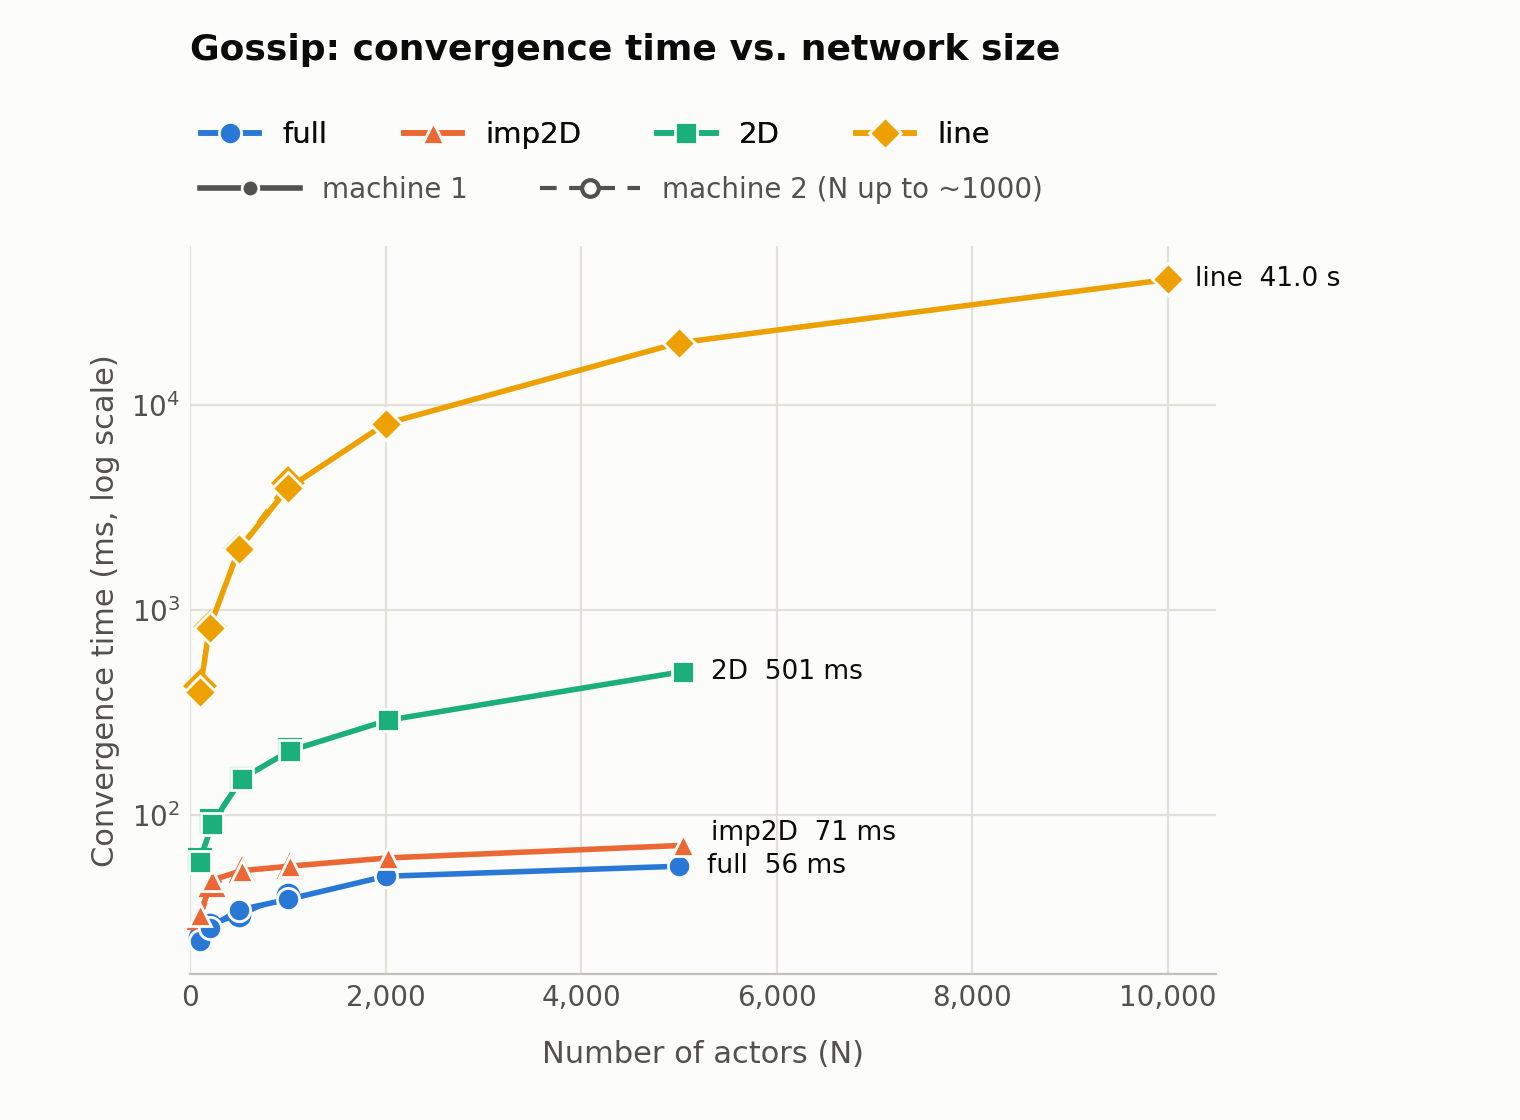
\includegraphics[width=0.6\textwidth]{gossip_plot_both_runs.png}
\caption{Gossip Results}
\end{figure}

\subsubsection*{Push-Sum Algorithm Results}
\begin{figure}[H]
\centering
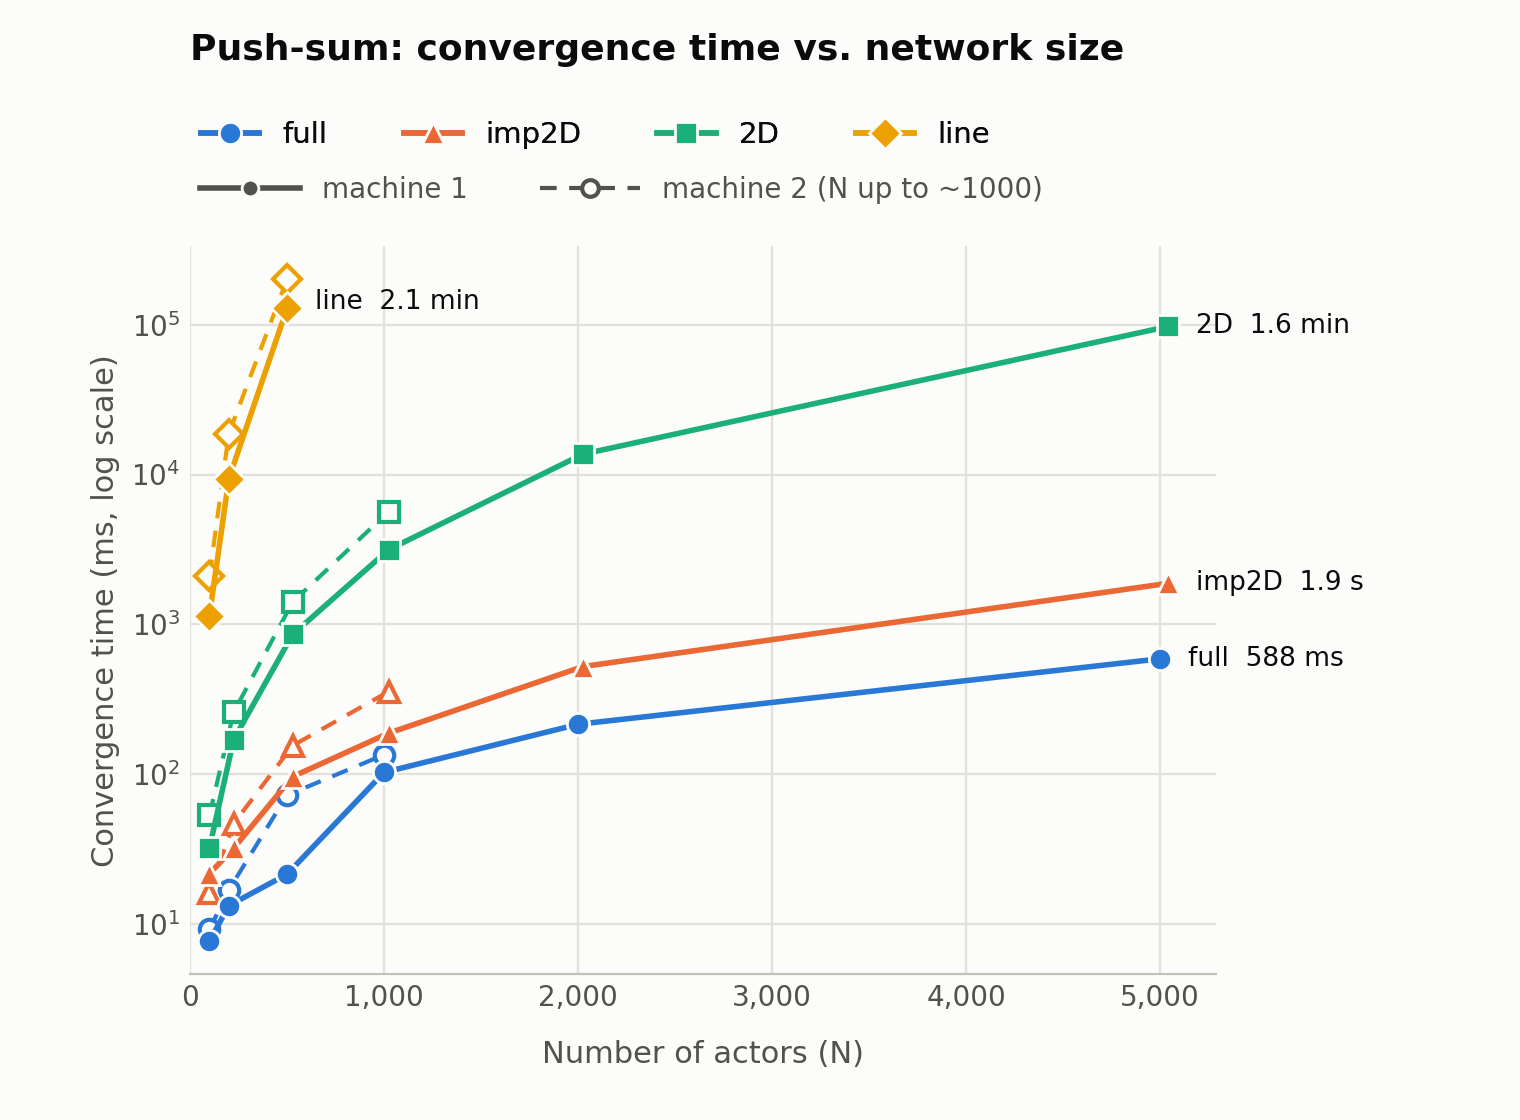
\includegraphics[width=0.6\textwidth]{pushsum_plot_both_runs.png}
\caption{Push-Sum Results}
\end{figure}

\subsubsection*{Summary of all the runs}
\begin{table}[H]
\centering
\begin{tabular}{llrrr}
\toprule
Algorithm & Topology & Largest $N$ run & Time at largest $N$ & Growth exponent$^{*}$ \\
\midrule
gossip   & full  & 5000  & 56 ms    & 0.22 \\
gossip   & imp2D & 5041  & 71 ms    & 0.18 \\
gossip   & 2D    & 5041  & 501 ms   & 0.54 \\
gossip   & line  & 10000 & 41.0 s   & 1.00 \\
\midrule
push-sum & full  & 5000  & 588 ms   & 1.16 \\
push-sum & imp2D & 5041  & 1.9 s    & 1.17 \\
push-sum & 2D    & 5041  & 97.5 s   & 2.03 \\
push-sum & line  & 500   & 128.5 s  & 2.93 \\
\bottomrule
\end{tabular}

\vspace{1ex}
{\footnotesize $^{*}$Slope of a least-squares fit of $\log(\mathrm{time})$ against $\log(N)$ over all machine 1 data points, i.e.\ time $\propto N^{\mathrm{exponent}}$.}
\caption{Summary of All Runs (machine 1)}
\end{table}


\section{Finding}
\textbf{Topology ordering is the same for both algorithms:} full is fastest, then imp2D, then 2D, and the line is
slowest. The better connected the network, the faster information mixes.
\textbf{Gossip on a line grows linearly} (exponent 1.00, about 4 ms per actor, 41 s at N=10000). The rumor can
only move one hop at a time, so the time is proportional to the length of the line.
\textbf{Gossip on full and imp2D grows very slowly} (exponents 0.22 and 0.18; roughly logarithmic). Going
from 100 to 5000 actors only about doubles the time for full. Plain 2D grows faster (exponent 0.54, since
the grid diameter is about the square root of N).
\textbf{One random extra link makes a huge difference.} imp2D has only one more neighbor than 2D, but at
N=5041 it is about 7x faster for gossip (71 ms vs 501 ms) and about 50x faster for push-sum (1.9 s vs 97
s).
\textbf{Push-sum scales much worse than gossip on sparse topologies.} The exponent is about 2.0 for 2D
and about 2.9 for the line (1.1 s at N=100, 9.4 s at N=200, 129 s at N=500), against about 1.2 for full and
imp2D. In push-sum every actor's ratio must settle, not just receive one message, and only one message
is in flight at a time, so the pairs have to diffuse slowly across a poorly connected network.
\textbf{Largest networks:} gossip reached N=10000 on the line and N=5000 or more on the others; push-sum
reached N=5000 on full, 5041 on imp2D and 2D, and N=500 on the line (It was taking more than 20 minutes on N=1000).

\section{Caveats}
All measurements for the report and the README come from one machine \textbf{Macbook Pro M3 Pro} , so absolute times depend on the hardware and on how the
Erlang scheduler shares cores among thousands of processes. Only 3 runs were averaged per point, so
small differences (especially at small N) are noise. Gossip times include the 1 ms send timer, which sets a
floor of a few milliseconds per hop of the spread.

The measurements in the dashed plot comes from \textbf{Macbook Pro M1 Pro}. We decided to show plots on both of our machines to see differences and similarities in the plot due to different CPU chips.

\end{document}